\section{Mapserver Peta Bali}
MapServer  adalah aplikasi freeware dan Open Source digunakan untuk  menampilkan GIS di web. Salah satunya adalah penggunaan Mapserver pada Peta Bali karena sudah tersedia pada web Mapserver. Cara menjalankan aplikasi tersebut perlu menginstall MS4W.
Mapzen dibangun dari berbagai peralatan open-source yang dikemas ke dalam layanan Web dan di hosting di server Mapzen. Salah satu keunggulan Mapzen selain keterbukaannya adalah penggunaan mesin rendering fleksibel yang disebut Tangram untuk menampilkan peta digital dalam nuansa 2D maupun 3D secara real-time, sehingga membuat kartografi akan terlihat bagus dimana-saja.
MS4W ini dapat digunakan pada windows dalam menjalan Mapserver Bali tersebut. Disini akan dijelaskan cara instalasi, proses penggunaan MapServer pada Peta Bali, dan Hasil Proses yang sudah dijalankan tersebut.
\subsection{Cara Instalasi Mapserver}
\begin{enumerate}
\item
Download Mapserver atau disingkat MS4W di http://mapserver.org/download.html \ref{gambar1} seperti gambar dibawah ini
\begin{figure}[ht]
	    \centerline{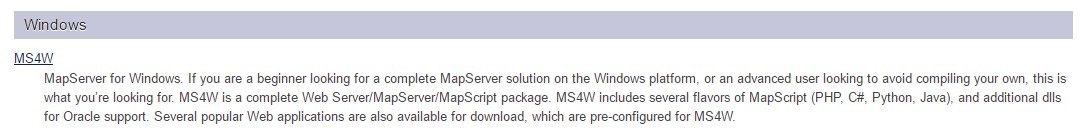
\includegraphics[width=0.50\textwidth]{figures/gambar1.JPG}}
	    \caption{Download MS4W}
		\label{gambar1}
		\end{figure}
\item
Setelah di download jalankan setupnya, disini saya menggunakan port 8080 karena port default 80 sudah dipakai oleh xampp \ref{gambar2} seperti gambar dibawah ini
\begin{figure}[ht]
	    \centerline{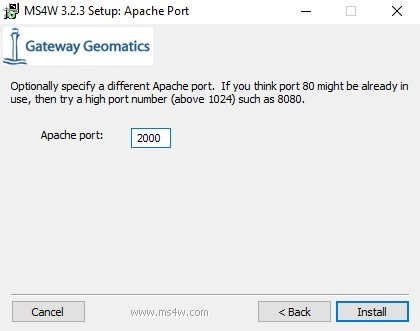
\includegraphics[width=0.50\textwidth]{figures/gambar2.JPG}}
	    \caption{Port 2000}
		\label{gambar2}
		\end{figure}
\item
Lalu tunggu instalasi sampai selesai \ref{gambar3} seperti gambar dibawah ini
\begin{figure}[ht]
	    \centerline{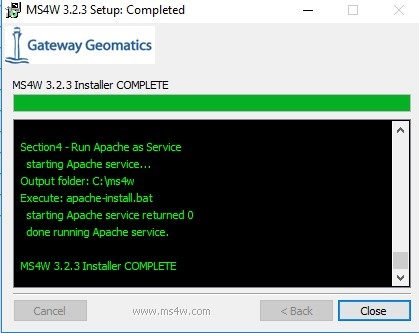
\includegraphics[width=0.50\textwidth]{figures/gambar3.JPG}}
	    \caption{Selesai}
		\label{gambar3}
		\end{figure}
\item
Setelah proses selesai silahkan buka browser favorit anda, kemudian ketikkan http://localhost:8080 di kotak isian URL.
\item
Jika anda melihat tampilan home MAPSERVER atau MS4W proses instalasi anda berhasil \ref{gambar4} seperti gambar dibawah ini
\begin{figure}[ht]
	    \centerline{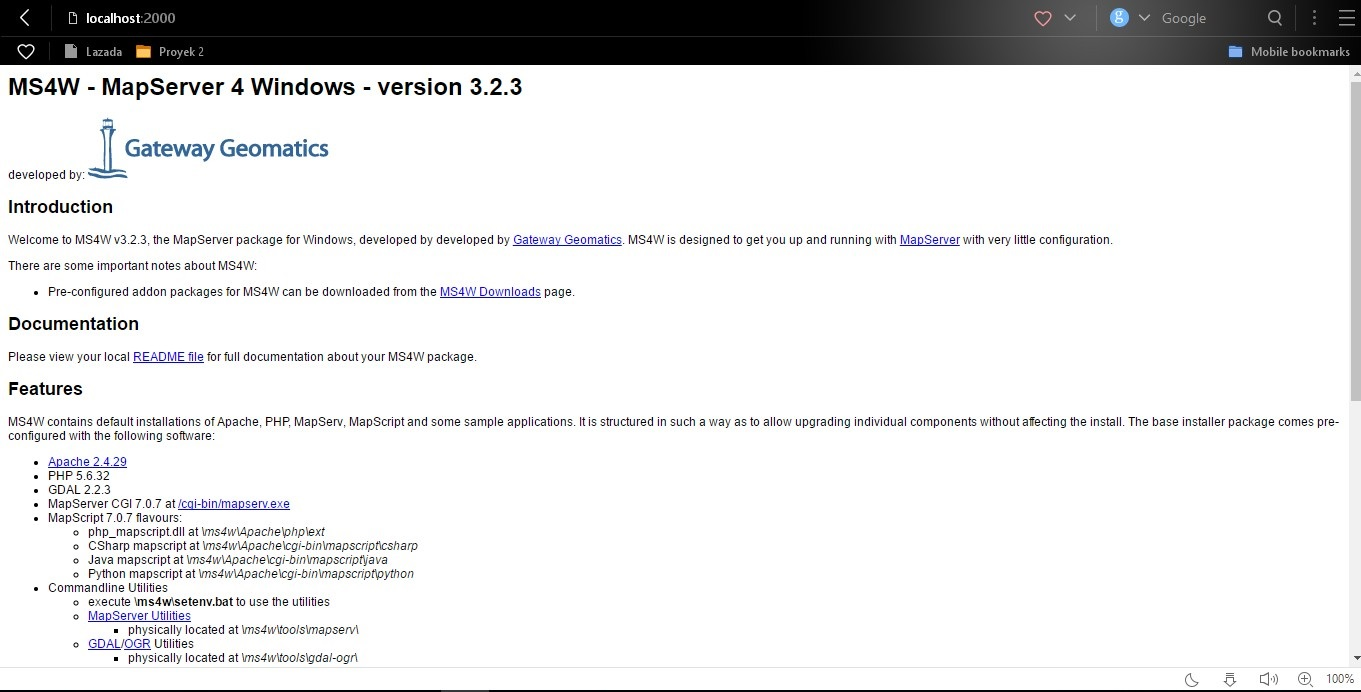
\includegraphics[width=0.50\textwidth]{figures/gambar4.JPG}}
	    \caption{Tampilan MS4W}
		\label{gambar4}
		\end{figure}
\end{enumerate}
Sekian Proses instalasi Mapserver pada Windows
